\documentclass[a4paper,10pt]{beamer}
\usepackage[utf8x]{inputenc}
\usepackage[T1]{fontenc}
\usepackage[english]{babel}
\usepackage{hyperref,graphicx,multicol,eurosym}
\usetheme{Berkeley}

\setbeamertemplate{navigation symbols}{\large \insertframenumber /\inserttotalframenumber}

\title{3D objects from 2D drawings}
\author[Groupe 3INFO]{Aurélien Fontaine, Manutea Huang, Etienne Geantet,\\ Arnaud Martin}
\institute[INSA de Rennes]{Institut National des Sciences Appliquées de Rennes}
\date{\today}

\begin{document}
	\begin{frame}
		\begin{titlepage}
			\centerline{
\includegraphics[scale=0.1]{images/logos/logoINSA.jpg}}
			\centerline{Tutors : François Lehericey and Bertrand Coüasnon}	
		\end{titlepage}
	\end{frame}
	
	
	
	\section{Introduction}
		\subsection{Existing technologies}
		
		\begin{frame}{A project made by Sony}
			Project PS4 : The PlayRoom (now available)
			\href{run:The_PlayRoom.avi}{
\includegraphics[width=300pt]{images/The-Playroom.jpg}}
		\end{frame}
		
			
	\begin{frame}
		\tableofcontents
	\end{frame}
			
		\subsection{Our subject}
		
		\begin{frame}{The subject}
			\begin{itemize}
				\item Create an object from a drawing on a tablet
			%\centerline{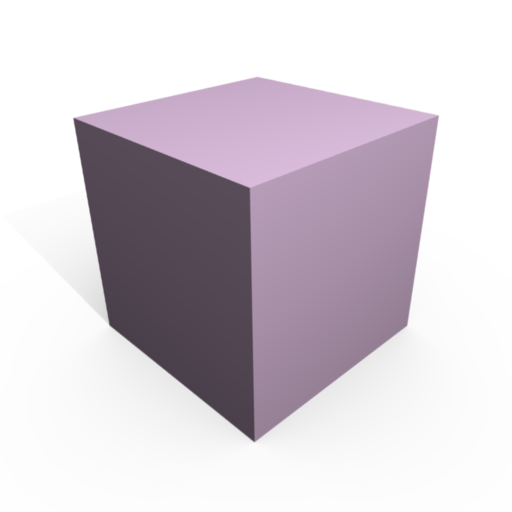
\includegraphics[height=100pt]{images/cube.png}
			%	\mbox{ }
			%
\includegraphics[height=100pt]{images/minute.jpg}}
				\item Easy to use: <1min to create a new object
			\end{itemize}
			%\centerline{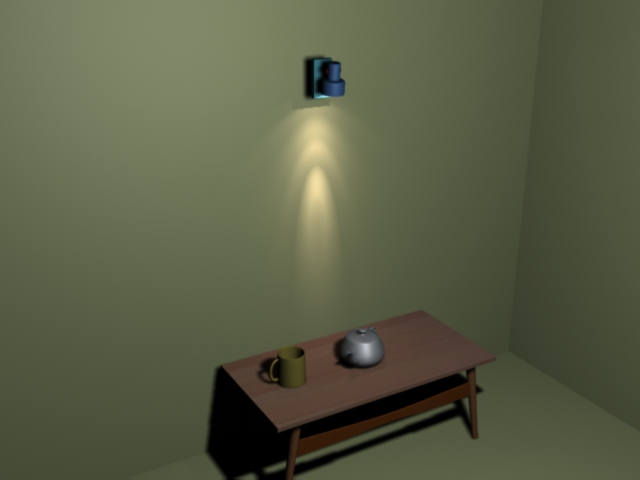
\includegraphics[height=100pt]{images/room.jpg}}              
			\underline{Final objective :} Occupy a room with simple objects made by a user
		\end{frame}
		
			\begin{frame}{Drawing editors}
				\begin{itemize}
					\item A lot of drawing editors : Markers, LayerPaint, SketchBook, ...
					\item Great drawings
					\item No possibility of making a 3D object
					\item Source code inaccessible
				\end{itemize}
			\end{frame}
	
	\section{Our solution}
		\subsection{Specifications}
		
		\begin{frame}{Specifications}
			\begin{itemize}
				\item Tablet application
				\item Create more or less complex 3D objects
				\item Ergonomic application
				\item The exportation: Unity compatible
			\end{itemize}
		\end{frame}
		
		\subsection{The interface}
		
			\begin{frame}{The app}
				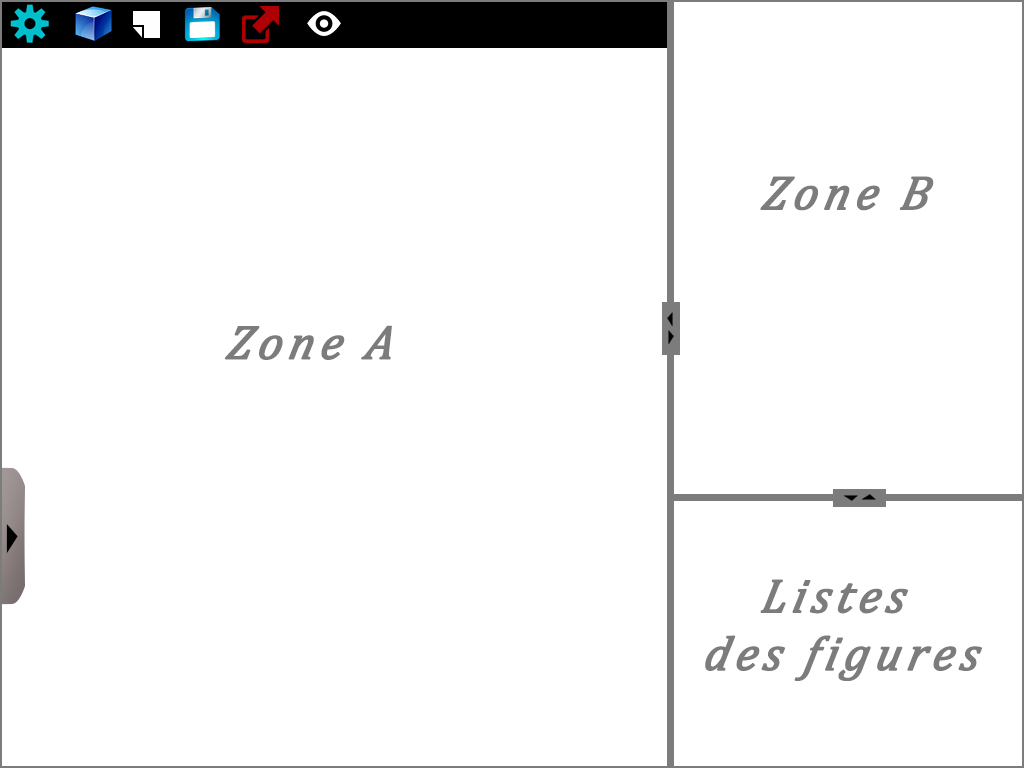
\includegraphics[height=205pt]{maquette/maquette_1.png}
			\end{frame}
			
			\begin{frame}{The app}
				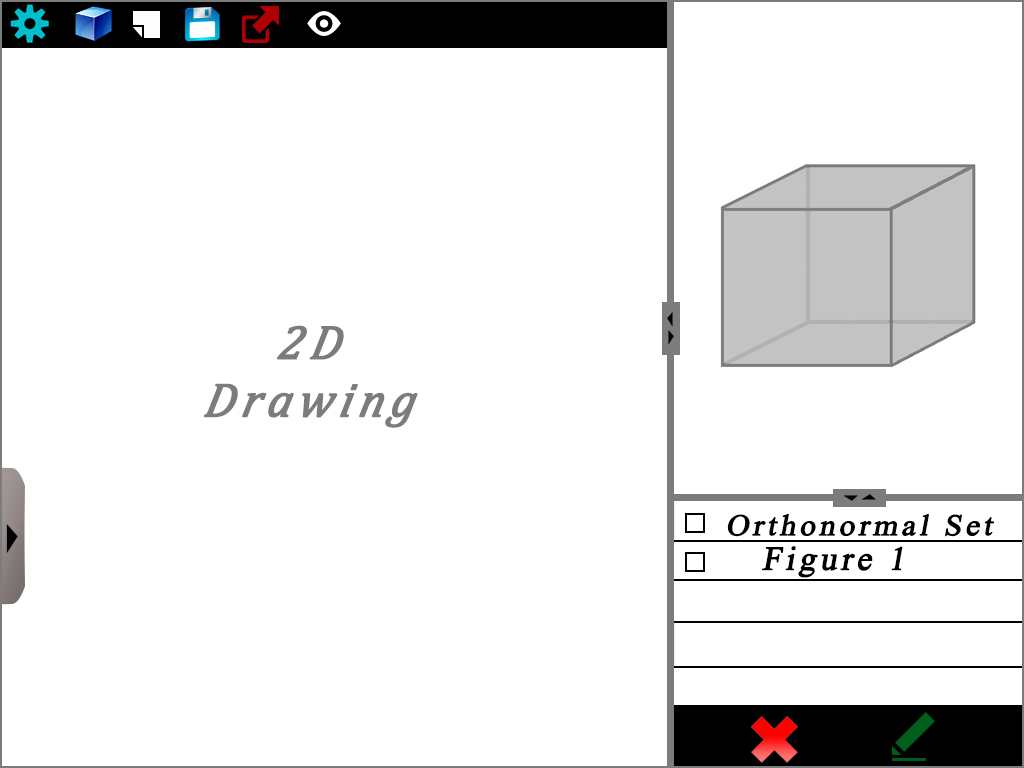
\includegraphics[height=205pt]{maquette/maquette_2.png}
			\end{frame}
			
			\begin{frame}{The app}
				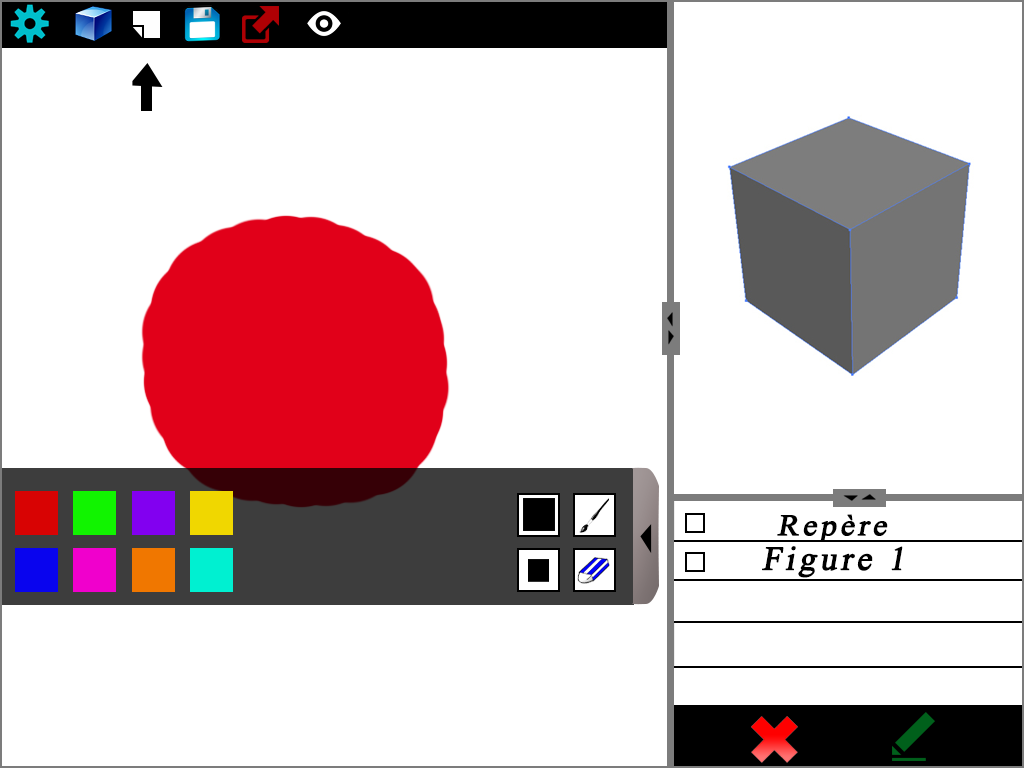
\includegraphics[height=205pt]{maquette/maquette_3.png}
			\end{frame}
			
			\begin{frame}{The app}
				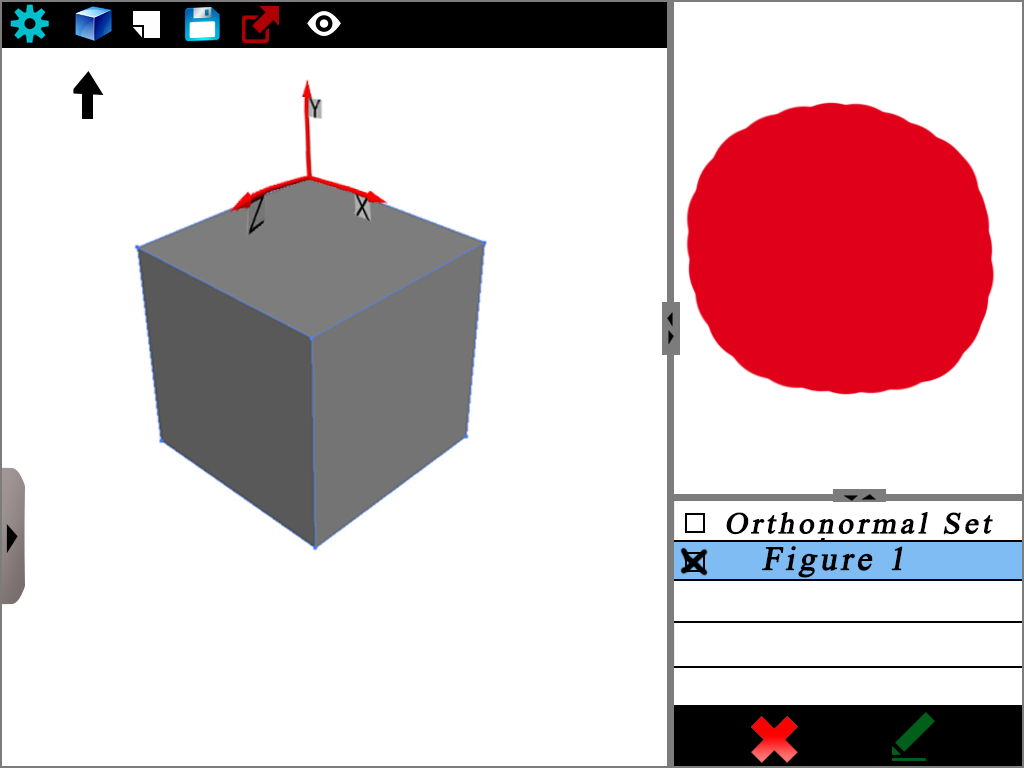
\includegraphics[height=205pt]{maquette/maquette_4.png}
			\end{frame}
			
			\begin{frame}{The app}
				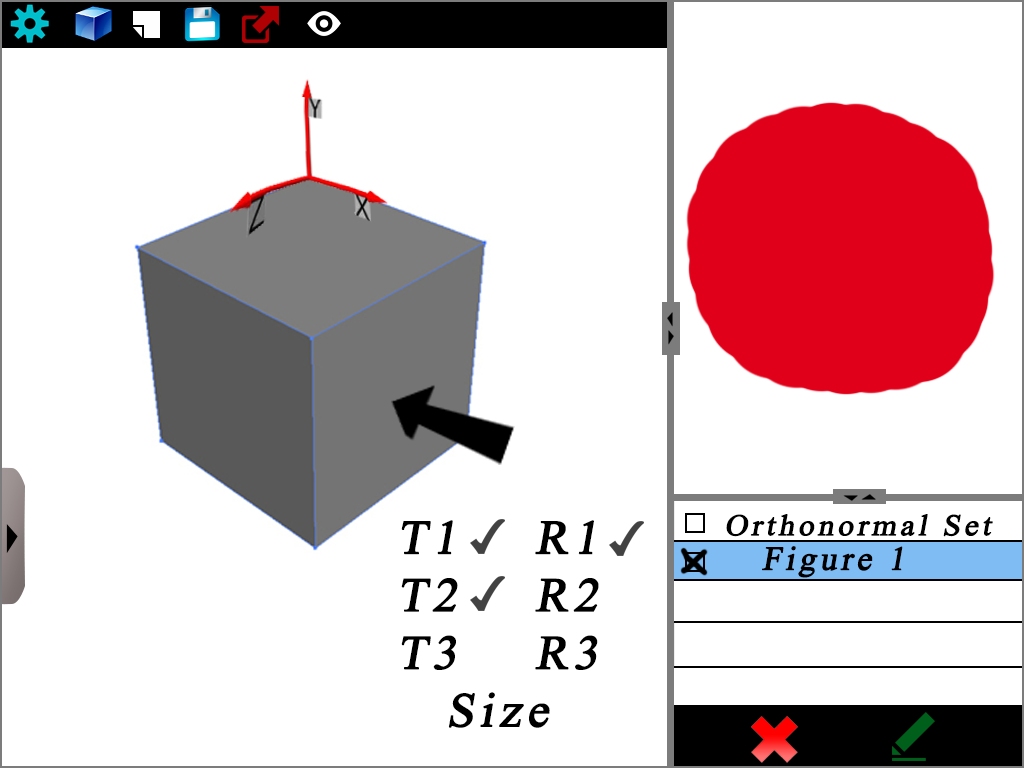
\includegraphics[height=205pt]{maquette/maquette_5.png}
			\end{frame}
			
			\begin{frame}{The app}
				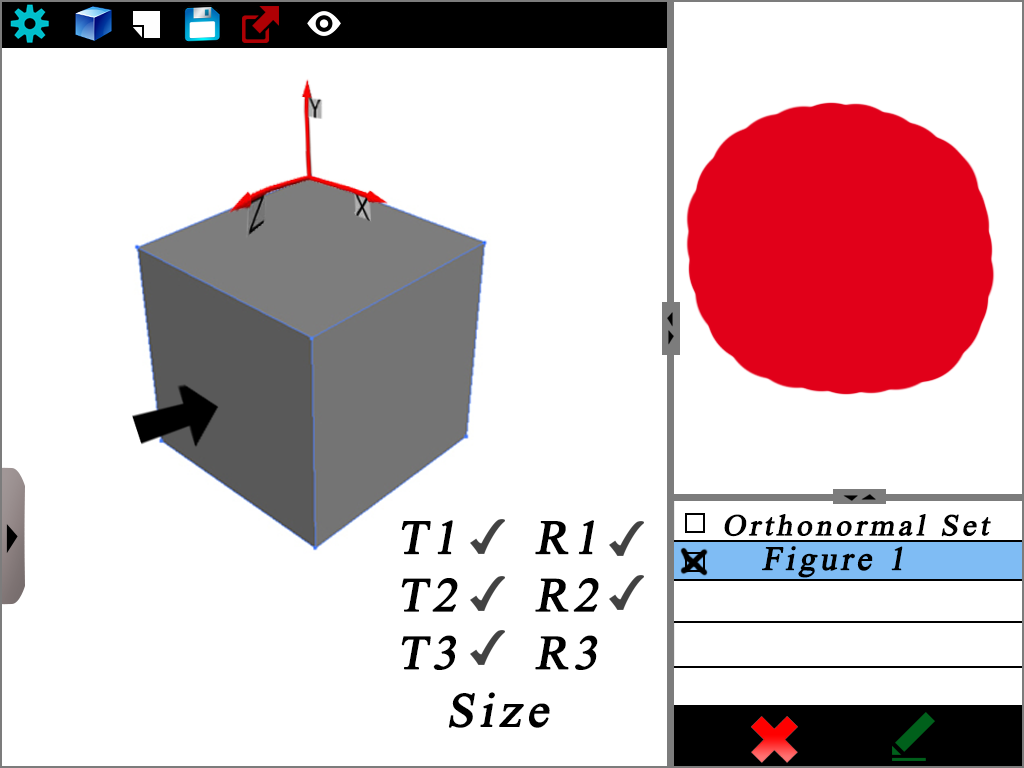
\includegraphics[height=205pt]{maquette/maquette_6.png}
			\end{frame}
			
			\begin{frame}{The app}
				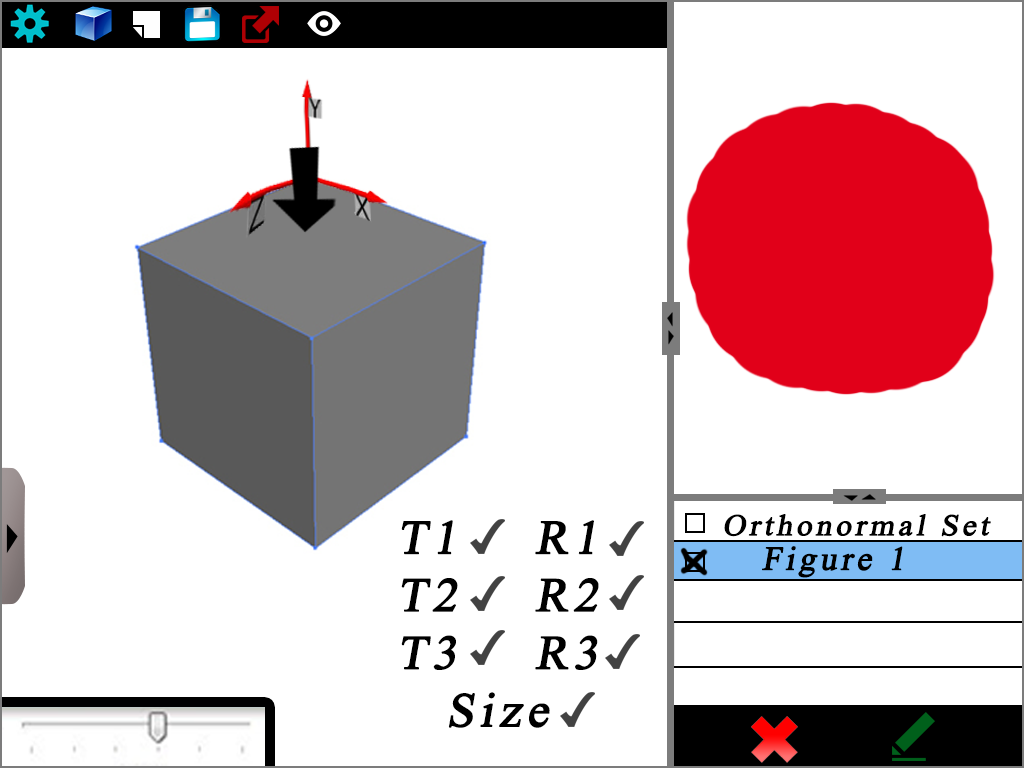
\includegraphics[height=205pt]{maquette/maquette_7.png}
			\end{frame}
			
			\begin{frame}{The app}
				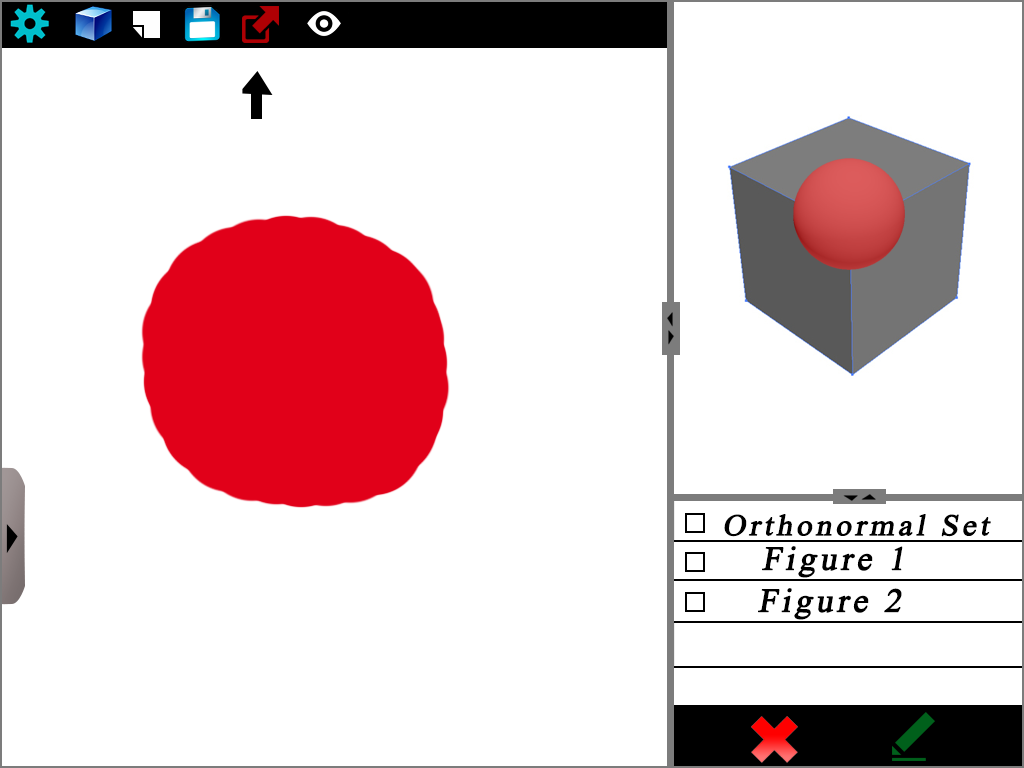
\includegraphics[height=205pt]{maquette/maquette_8.png}
			\end{frame}
			
		\subsection{Network}
		
			\begin{frame}{Network}
			\centerline{
\includegraphics[height=205pt]{images/network/network.png}}
			\end{frame}
			
			\subsubsection{How will it work?}
			
			\begin{frame}{How will it work?}
				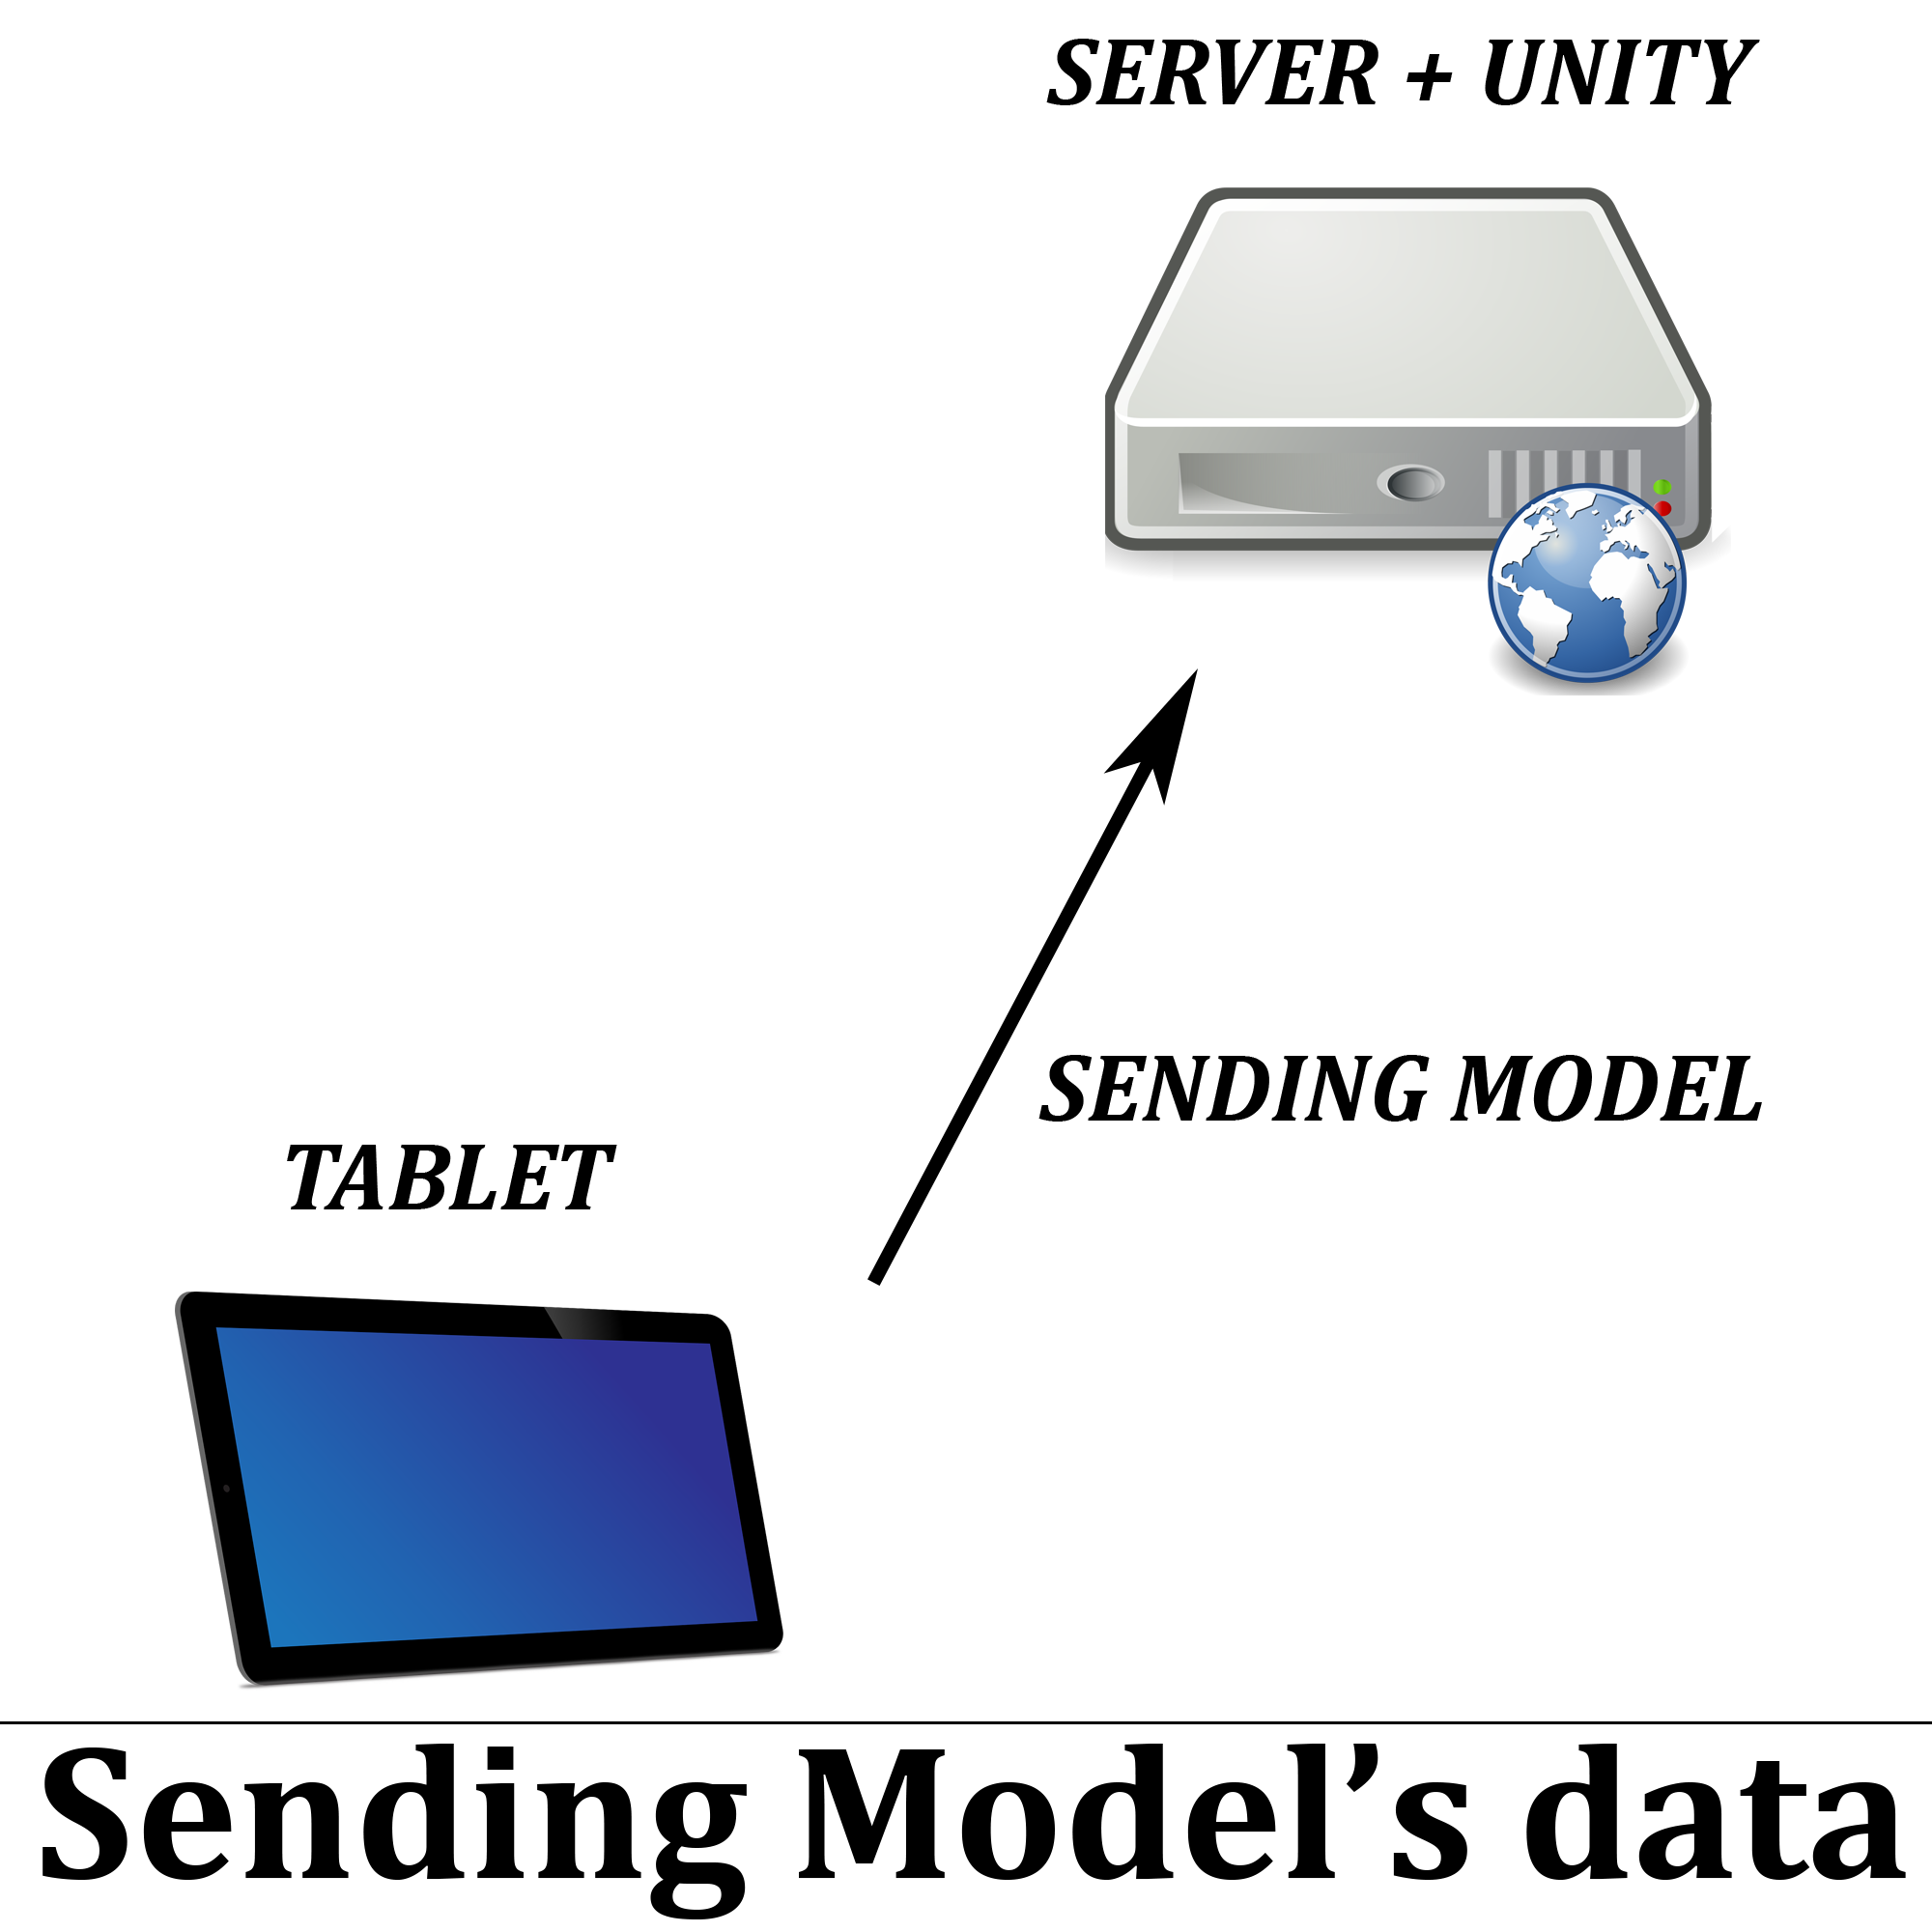
\includegraphics[height=100pt]{images/network/sending_model.png}\hspace{50pt}\pause
\includegraphics[height=100pt]{images/network/plugin.png}
				
				\hspace{150pt}
				Simple

				\hspace{150pt}
				Few lines
				
			\end{frame}
			
			\subsubsection{External Application?}
			
			\begin{frame}{External Application?}
				\centerline{
\includegraphics[height=100pt]{images/network/no.png}}
				\begin{itemize}
					\item HTTP (HyperText Transfert Protocol)
					\item FTP (File Transfert Protocol)
				\end{itemize}
			\end{frame}
			
			\subsubsection{Framework}
			
			\begin{frame}{Framework}
				\centerline{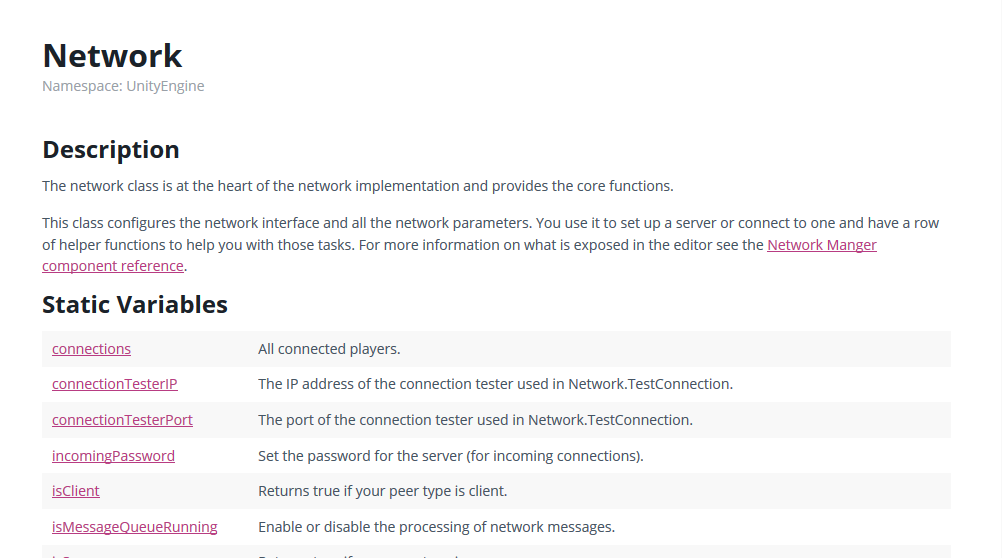
\includegraphics[height=150pt]{images/network/networkclass.png}}
			\end{frame}
		
	\section{The technology : the engine}
			
			\begin{frame}{The technology}
				How could we make our application ?
				\begin{itemize}
					\item FPS (First-person shooter) game engines
					\item API (Application Programming Interface)

				\end{itemize}
			\end{frame}
			
		\subsection{FPS game engines}
		
			\begin{frame}{Unreal engine}
				\begin{multicols}{2}
				
\includegraphics[height=100pt]{images/logos/Unreal_Engine.png}\\
				
				\columnbreak 
				
				 \begin{itemize}
				 	\item \underline{Use :}\\		
					 FPS game engine	 
					 \item \underline{Qualities :}\\
						 \begin{itemize}
						 	\item Can work with a lot of objects
						 	\item Easy to use : C++
						 \end{itemize}
				 \end{itemize}		 
				\end{multicols}
				\begin{itemize}
					\item \underline{Defaults :}\\
					\begin{itemize}
						\item View FPS inevitable
						\item A sand box for game
						\item Lack of tools to develop on tablets
						\item Licence expensive (19\euro/month + 5\%)
					\end{itemize}
				\end{itemize}
			\end{frame}
			
			\begin{frame}{CryEngine}
				\begin{multicols}{2}
					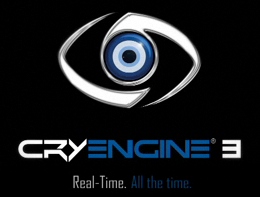
\includegraphics[height=100pt]{images/logos/Cry_Engine.png}\\
					
					\columnbreak 
					
					\begin{itemize}
						\item \underline{Use :}\\		
						FPS game engine				
						\item \underline{Qualities :}\\
						\begin{itemize}
							\item Can work with a lot of objects
							\item Easy to use : C++
							\item Cross platform
						\end{itemize}
					\end{itemize}		 
				\end{multicols}
				\begin{itemize}
					\item \underline{Defaults :}\\
					\begin{itemize}
						\item View FPS inevitable
						\item A sand box for game
						\item Lack of tools to develop on tablets
						\item Licence expensive (9.99\euro/month)
					\end{itemize}
				\end{itemize}
			\end{frame}
			
			
		\subsection{Others API}
		
			\begin{frame}{OpenGl}
				\begin{multicols}{2}
					
\includegraphics[height=70pt]{images/logos/OpenGL_logo.png}\\
					
					\columnbreak 
					
					\begin{itemize}
						\item \underline{Use :}\\		
						Hardware oriented language			
						\item \underline{Qualities :}\\
						\begin{itemize}
							\item Need few resources
						\end{itemize}
					\end{itemize}		 
				\end{multicols}
				\begin{itemize}
					\item \underline{Defaults :}\\
					\begin{itemize}
						\item New language
						\item Hard to create a simple object
						\item Hard to move to different devices
						\item OpenGl ES : less functions than OpenGl
					\end{itemize}
				\end{itemize}
			\end{frame}
			
			\begin{frame}{Autodesk Maya}
				\begin{multicols}{2}
					
\includegraphics[height=60pt]{images/logos/Autodesk_Maya.png}\\
					
					\columnbreak 
					
					\begin{itemize}
						\item \underline{Use :}\\		
						3D computer graphics software		
						\item \underline{Qualities :}\\
						\begin{itemize}
							\item Easy to use : C++
							\item Very rich library
						\end{itemize}
					\end{itemize}		 
				\end{multicols}
				\begin{itemize}
					\item \underline{Defaults :}\\
					\begin{itemize}
						\item Very expensive licence (\$185.00/month)
						\item Made for specials effects in films
					\end{itemize}
				\end{itemize}
			\end{frame}
		
			\begin{frame}{Unity}
				\begin{multicols}{2}
					
\includegraphics[height=80pt]{images/logos/Logo_Unity.jpg}\\
					
					\columnbreak 
					
					\begin{itemize}
						\item \underline{Use :}\\		
						Cross-platform game creation system 		
						\item \underline{Qualities :}\\
						\begin{itemize}
							\item Easy to export to an Unity server
							\item Easy to use : C\#
							\item Lots of help for tablet development
							\item Very rich library
							\item Free
						\end{itemize}
					\end{itemize}		 
				\end{multicols}
				\begin{itemize}
					\item \underline{Defaults :}\\
					\begin{itemize}
						\item None
					\end{itemize}
				\end{itemize}

			\end{frame}
			
		

	
	\section{Conclusion}
	
		\begin{frame}{Conclusion}
			\centerline{
\includegraphics[height=100pt]{images/conclusion/loupe.png}}
			\begin{itemize}
				\item Modify the interface ?
				\item improve knowledge on the Network class
			\end{itemize}
		\end{frame}
\end{document}
